\section{acceleraTor Design and Implementation}
\label{sec:design}

In this section we describe acceleraTor's design in some detail and briefly 
explain relevant implementation issues.

\subsection{Design Overview}
\label{subsec:design-overview}

acceleraTor's overall design is depicted in Figure~\ref{fig:accelerator-design}: we 
compare it with the design of `vanilla' Tor to clearly emphasize their differences.

\begin{figure}[h!]

    \centering
    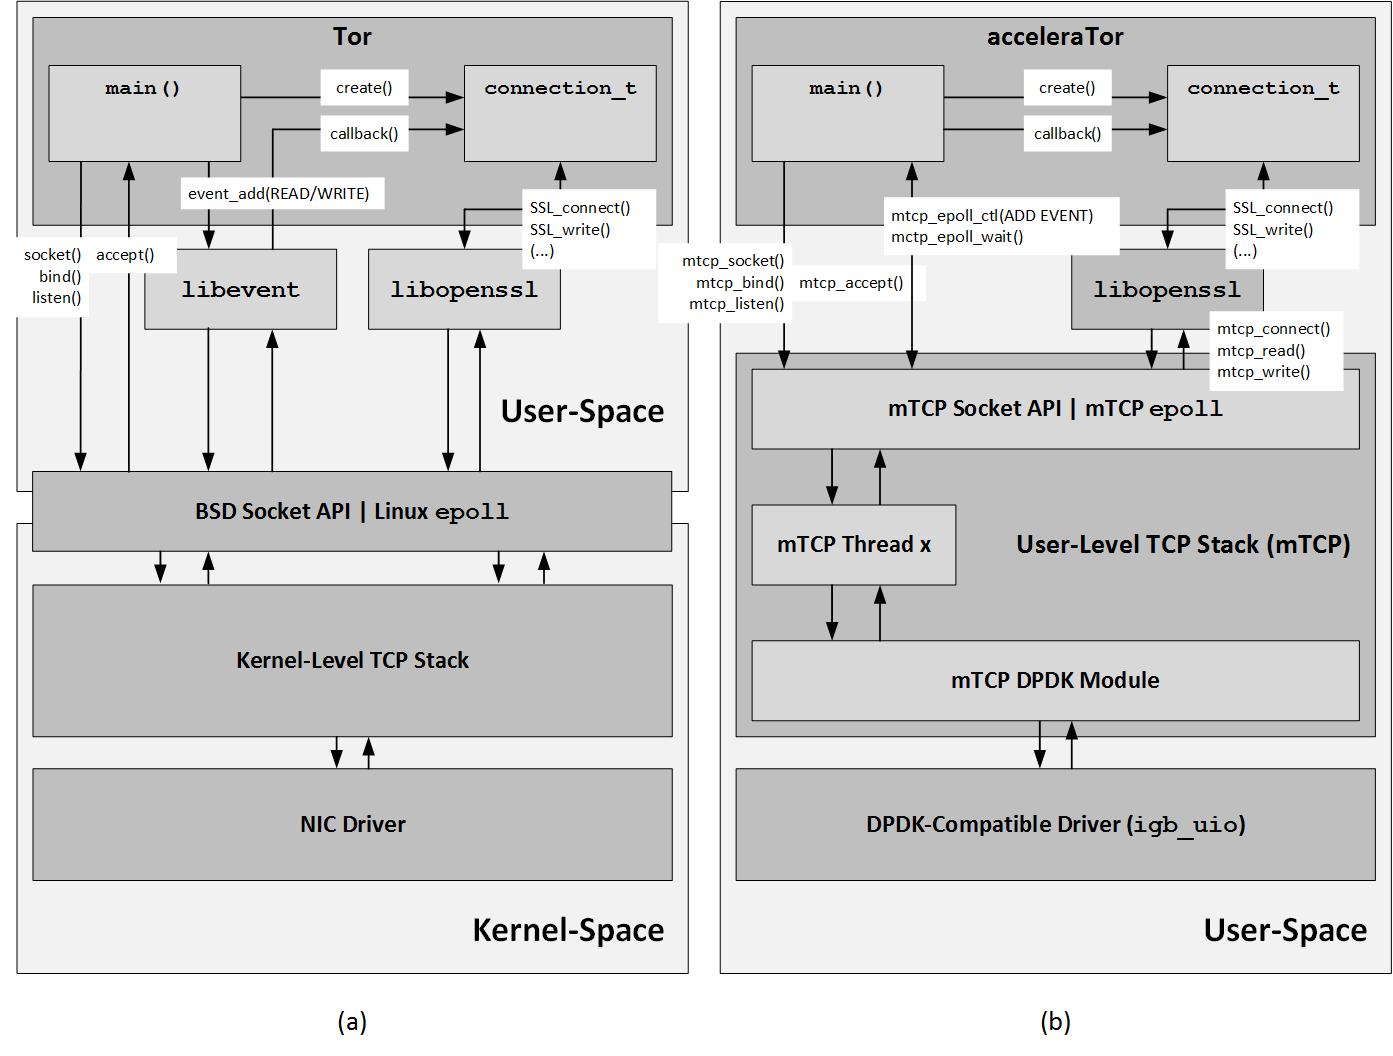
\includegraphics[width=0.50\textwidth]{figures/design.png}
    \cprotect\caption{`Vanilla' Tor (a) vs. acceleraTor's (b) design overview.}
    \label{fig:accelerator-design}

\end{figure}

At the extremes (top and bottom) we have acceleraTor as a TCP-based network 
application which implements Tor OR application logic and the 
pre-defined user-level packet input\slash output 
(I\slash O) library, DPDK v1.8, which reads\slash writes packets directly 
from DPDK-compatible Network Interface Cards (NICs), at user-level. 
The main difference with respect to `vanilla' Tor is that all levels in 
acceleraTor's design run in user space. In-between, we recur to a user-level 
TCP stack -- mTCP~\cite{179773} -- to neatly interconnect acceleraTor and DPDK, 
and ultimately reserve the `services' of 
a single DPDK-compatible NIC to the application. Although not 
part of acceleraTor's design per se, due to this 
application-NIC `exclusivity', we run acceleraTor in nodes equipped with 
two NICs, one to be handled by a DPDK-compatible driver and reserved for 
acceleraTor, another handled by a kernel driver, which allows for the parallel operation of `usual' 
networking applications.

In the next subsections, we discuss design and implementation aspects for each 
one of the levels in more detail.

\subsection{Tor's Integration with mTCP}
\label{subsec:design-mtcp}

Some of the benefits brought about by DPDK come from a bypass of the kernel 
networking stack, allowing applications to process `raw' packets at the 
user-level and thus overcome kernel-level inefficiencies such as heavy system 
call overhead~\cite{179773, Brouer2014}. Nevertheless, such a `bypass' also 
involves challenges. Without kernel-level support of TCP, we either: 

\begin{enumerate}
	\item Modify Tor to become independent of TCP, having it directly process 
		packets `fresh' out of the NICs;
	\item Develop\slash use an user-level TCP stack, integrated with DPDK, on 
		top of which Tor can be adapted.
\end{enumerate}

Option 1 would heavily modify the way Tor 
works -- e.g. Tor makes heavy use of TLS, which depends on TCP's reliable transport -- not 
only making acceleraTor ORs incompatible with `vanilla' Tor nodes, 
but also making acceleraTor's modifications to Tor unnecessarily intrusive and harder. Option 2 is 
more desirable: ideally, it should rely on an intermediate module which (1) interfaces with 
DPDK to read\slash write `raw' packets from\slash to NICs, (2) implements ``enough of'' TCP to 
have TCP-based applications and TLS work on top of it; and (3) exposes a 
`BSD-like' socket API, allowing for easy integration of TCP-based applications 
and libraries (e.g. OpenSSL\footnote{\url{https://openssl.org/}} for TLS).

mTCP~\cite{179773} is a user-level TCP stack which -- while specifically 
designed to solve TCP performance issues in multicore systems -- fulfills the 
points of the `ideal' option 2: as of version 3\footnote{Released in 
April 2, 2015, \url{https://github.com/eunyoung14/mtcp}.}, mTCP comes directly 
integrated with DPDK (v1.8 and v2.0). Other choices have been quickly 
surveyed -- e.g. drv-netif-dpdk\footnote{https://github.com/rumpkernel/drv-netif-dpdk}, a 
DPDK interface for Rump Kernels~\cite{Rump2015}; the solution proposed by Kantee 
et al. in~\cite{Kantee2009}; or NUSE~\cite{Nuse2015} -- but dismissed since these 
could not beat mTCP's suitability to the aforementioned requirements.

Despite its convenience, the use mTCP to integrate Tor and DPDK poses the 
following set of implementation challenges, some of which are briefly addressed 
in the following subsections:

\begin{itemize}
	\item mTCP's API slightly differs from the `BSD' socket API used in Tor, and 
		does not provide all its functionalities. acceleraTor must accommodate 
		these limitations without major loss of functionality.
	% \item mTCP supports only one listening socket 
	% 	per `mTCP thread'. In addition, (...). Therefore, acceleraTor must 
	% 	demultiplex OR connections, which are given independent 
	% 	listening sockets in the `vanilla' version of Tor.
	\item In its `vanilla' version, Tor makes use 
		of \verb+libevent+\footnote{\url{http://libevent.org/}} to handle 
		asynchronous input\slash output (IO). mTCP provides 
		its own \verb+epoll+-like event system to monitor mTCP sockets, not 
		compatible with \verb+libevent+\cprotect\footnote{I.e. \verb+libevent+ does not 
		recognize the event-checking `method' made available 
		by mTCP's event system.}. Therefore, Tor's asynchronous IO logic must 
		be changed.
	\item Tor makes heavy use of Transport Layer Security (TLS) connections, 
		through OpenSSL, which must 
		now be modified to comply with mTCP's API.
\end{itemize}

\subsubsection{Porting Tor to mTCP}
\label{subsubsec:design-mtcp-port}

Since mTCP provides a `BSD-like' socket API, most of the porting effort 
consisted in identifying the code using `BSD-like' system calls and 
replacing these mTCP's equivalent calls. Such changes have been kept as 
contained and isolated as possible: we allow for the selective  
compilation of either `vanilla' Tor or acceleraTor via a new 
Tor configuration option\footnote{Source code and setup scripts available 
at \url{https://bitbucket.org/clockWatchers/accelerator}}.

Besides `syscall-translation', the porting effort also included the 
initialization of a single mTCP thread from within Tor's main thread, 
which ultimately `binds' to an available DPDK-compatible NIC. Tor's main loop 
was changed to continuously wait for mTCP events (e.g. new connections, 
read\slash write events on existing connections) using mTCP's user-level event 
system : in Tor's original design, a similar approach is used to listen for 
new events, using \verb+libevent+'s API instead. More details are given in 
section~\ref{subsubsec:design-mtcp-event}.

% \subsubsection{Connection De-Multiplexing}
% \label{subsubsec:design-mtcp-demultiplex}

\subsubsection{Event Handling Logic}
\label{subsubsec:design-mtcp-event}

Tor uses asynchronous input\slash output (IO) to monitor sockets 
associated with inter-OR TCP connections and invoke appropriate connection-handling 
callbacks whenever read\slash write events are triggered. mTCP provides 
its own \verb+epoll+-like event system to monitor mTCP connections, not 
compatible with \verb+libevent+, used by `vanilla' Tor.

When adding creating a new OR\slash client connection, Tor registers new read\slash write 
events to monitor the file descriptors (i.e. sockets) associated with the 
connection. \verb+libevent+'s API allows 
for a direct association between the registered event and a 
specific connection descriptor. The same is not possible in mTCP: mTCP's API 
associates events with a socket file descriptor. We 
therefore need some `external' way of mapping socket file descriptors to the 
respective connection descriptor objects, and then re-use already existing 
read\slash write callbacks. We accomplish this via a global hash 
table, implemented 
using \verb+uthash+\footnote{\url{http://troydhanson.github.io/uthash/}}.

\subsubsection{Integration with OpenSSL}
\label{subsubsec:design-mtcp-openssl}

Last -- but definitely not least -- there is the issue of TLS: Tor 
makes heavy use of TLS to secure OR\slash client connections, and in turn uses 
OpenSSL's API to get TLS support. OpenSSL must then be also ported to mTCP. 
As OpenSSL's implementation relies on `BSD'-like system calls, the porting 
effort mostly consists in tracking down the code which uses such system calls 
and replace them with those exposed by mTCP API. Besides the `translation' effort, 
we introduce the changes in OpenSSL's API:

\textbf{a)} Added a new attribute in SSL structures (i.e. representations of a TLS 
connection), \verb+mctx_t mctx+, which represents the mTCP thread context to 
which the SSL structure should be associated with.

\textbf{b)} Added a new call to OpenSSL's API
\[\verb+int SSL_set_mtcp_ctx(SSL * s, mctx_t mctx)+\]
which lets accelaraTor (or other mTCP-based applications willing to use OpenSSL) 
set the mTCP thread context attribute on some SSL structure \verb+s+. These 
changes are convenient, as other calls exposed by OpenSSL's 
API -- e.g. \verb+SSL_connect(SSL * s)+ -- which 
originally only take a single SSL structure as argument, do not have to be 
changed to include an additional reference to the respective mTCP context as 
argument. This eases the integration effort on Tor's own source code (`wrapper' 
functions for OpenSSL's API, defined in \verb+tortls.c+).
%Unfortunately, this step could not 
%be fully completed by the end of the project's timeline, which compromised the 
%possibilities of having a working acceleraTor prototype by the end of the 
%project. %% don't know if this 
% should be included here or in a subsequent section...
% For the sake of completeness, we note that -- as an alternative to the 
% integration with a user-level TCP stack -- we may have had considered other 
% options such as Datagram TLS (DTLS)~\cite{rfc4347} to allow for TLS-like 
% functionalities over `connectionless' protocols such as UDP. Of course, 

\subsection{mTCP and DPDK}
\label{subsec:design-dpdk}

As of version 3, mTCP comes directly integrated with DPDK (v1.8 and v2.0), and 
so the relevant issues during development were implementation-related, mostly 
consisting in finding compromises with (OS- and hardware-level) constraints 
imposed by both mTCP and DPDK.

\begin{itemize}
	\item DPDK-compatible mTCP (v3) could only work with the Linux-3.13.0 kernel (we have used 
		3.13.0-46-lowlatency, which comes with the \verb+uio+ kernel module installed 
		by default);
	\item We have tested setups in both 32- and 64-bit architectures: in the 
		latter case, DPDK's libraries had to be compiled as shared;
	\item DPDK is compatible with a limited set of NICs: we have successfully 
		tested DPDK with Intel 82545 EM\footnote{Oracle Virtual Box: \url{https://www.virtualbox.org/}.}and Intel 82599\cprotect\footnote{AWS EC2 \verb+c4.large+ instances.} Ethernet adapters.
\end{itemize}
